\documentclass[12pt]{article}

\usepackage{algorithm}
\usepackage{algpseudocode}
\usepackage{amsmath}
\usepackage{amsfonts}
\usepackage{float}
\usepackage{fancyhdr}
\usepackage{graphicx}
\usepackage{placeins}
\usepackage[colorlinks=true,linkcolor=blue, citecolor=red]{hyperref}
\usepackage{url}
\usepackage[top=.75in, left=.75in, right=.75in, bottom=1in]{geometry}
\usepackage{arydshln}
\usepackage[utf8]{vietnam}
\setlength{\headheight}{29.43912pt}

\usepackage{mathptmx}
% \graphicspath{PATH_TO_GRAPHIC_FOLDER}

\pagestyle{fancy}
\fancyfoot{}
\fancyfoot[R]{Page \thepage}

\lhead{
Báo cáo đồ án môn học
}
\rhead{
Trường Đại học Khoa học Tự nhiên - ĐHQG HCM\\
Khai thác ngữ liệu văn bản nâng cao (MTH089)
}
\lfoot{\LaTeX\ template by \href{https://github.com/trhgquan}{Quan, Tran Hoang}}

\newcommand{\coursename}{Khai thác ngữ liệu văn bản nâng cao (MTH089)}
\newcommand{\reportname}{Xây dựng ứng dụng trích xuất triệu chứng sử dụng mô hình ViHealthBERT}

\begin{document}

\begin{titlepage}
\newcommand{\HRule}{\rule{\linewidth}{0.5mm}}
\centering

\textsc{\LARGE đại học quốc gia tphcm}\\[1.5cm]
\textsc{\Large trường đại học khoa học tự nhiên}\\[0.5cm]
\textsc{\large khoa công nghệ thông tin}\\[0.5cm]
% \textsc{bộ môn công nghệ tri thức}\\[0.5cm]

\HRule \\[0.4cm]
{ 
\huge{\bfseries{Báo cáo Đồ án Môn học}}\\[0.5cm]
\large{\bfseries{Đề tài: \reportname}}
}\\[0.4cm]
\HRule \\[0.5cm]

\textbf{\large Môn học: \coursename}\\[0.5cm]

\begin{minipage}[t]{0.4\textwidth}
\begin{flushleft} \large
\emph{Học viên thực hiện:}\\
Trần Hoàng Quân (19120338) \\
Phạm Anh Việt \textsc{(20C11060)} \\
Nguyễn Đức Thuận \textsc{(21C11035)} \\
Nguyễn Thiện Dương \textsc{(21C12004)} \\
\end{flushleft}
\end{minipage}
~
\begin{minipage}[t]{0.4\textwidth}
\begin{flushright} \large
\emph{Giáo viên hướng dẫn:} \\
% Dr. James \textsc{Smith}
TS. Nguyễn Trường Sơn\\
TS. Nguyễn Tiến Huy
\end{flushright}
\end{minipage}\\[1cm]

{\large \today}\\[1cm]


\includegraphics[scale=.3]{img/hcmus-logo.png}\\[1cm] 

\vfill
\end{titlepage}


\tableofcontents
\pagebreak

\section{Mô hình ViHealthBERT}
\subsection{Tóm tắt nội dung bài báo}
Trong những năm gần đây, các mô hình ngôn ngữ (Language Models - LM) được xây dựng và ứng dụng rộng rãi trong lĩnh vực Xử lý ngôn ngữ tự nhiên (NLP), chúng cũng đạt được nhiều kết quả đáng chú ý. Đặc biệt, chất lượng các mô hình đơn ngữ được huấn luyện sẵn dành cho những ngôn ngữ ít tài nguyên ngữ liệu đã tăng đáng kể. Đáng lưu ý, mặc dù các mô hình ngôn ngữ cho miền chung (general-domain language models) rất đa dạng, nhưng có rất ít các mô hình ngôn ngữ đặc thù dành riêng cho một số lĩnh vực (specific-domain language models). Vì lí do đó, nhóm tác giả bài báo \textit{ViHealthBERT: Pre-trained Language Models for Vietnamese in Health Text Mining}\cite{minh-EtAl:2022:LREC} công bố bài báo với những đóng góp sau:
\begin{itemize}
\item Giới thiệu mô hình ViHealthBERT là mô hình ngôn ngữ Tiếng Việt đặc thù cho lĩnh vực y tế.
\item Giới thiệu các bộ ngữ liệu Acronym Disambiguation (AD) và Freqently Asked Question (FAQ) Summarization là các bộ ngữ liệu đặc thù cho lĩnh vực y tế.
\end{itemize}

% Các mô hình ngôn ngữ quy mô lớn gần đây cho thấy những thành tựu đáng kể trong các tác vụ xử lý ngôn ngữ tự nhiên (NLP) chính như Hệ thống hỏi đáp(Q\&A) và Tóm tắt nội dung văn bản (Raffel et al., 2020). Nhiều nghiên cứu đã phát hiện ra các mô hình ngôn ngữ đa ngôn ngữ đều có hiệu suất tốt hơn trong một loạt các nhiệm vụ liên tiếp song son nhau (downstream tasks) mà không cần xem xét tính chất ngôn ngữ của nó và rất nhiều ngôn ngữ có nguồn lực thấp được hưởng lợi từ điều này.

% Một số bài toán,công trình về áp dụng các mô hình NLP có thể kể đến như :
% \begin{itemize}
%   \item Bài toán nhận dạng tên thực thể (NER) bằng tiếng Việt : mBERT(Devlin et al., 2019) , ELECTRA(Clark et al., 2020), viBERT và vELECTRA(Bui et al., 2020)
%   \item Mô hình ngôn ngữ tiếng Việt dựa trên BERT quy mô lớn đầu tiên : PhoBERT (Nguyễn và Tuấn Nguyễn, 2020)
%   \item Mô hình ngôn ngữ trong lĩnh vực pháp lý , áp dụng hoặc truy xuất văn bản pháp luật tiếng Việt (2020)
% \end{itemize}
% Có thể thấy rằng hiện có rất nhiều công trình nghiên cứu về NLP trong các lĩnh vực, tuy nhiên các nghiên cứu mà giải quyết các nhiệm vụ dành riêng cho lĩnh vực với tiếng Việt vẫn còn rất ít, vì các nghiên cứu về mô hình ngôn ngữ tiếng Việt hiện tại vẫn tập trung vào lĩnh vực chung chung
% Trong lĩnh vực y tế ,chăm sóc sức khỏe việc tận dụng các mô hình NLP đã được đào tạo trước của các lĩnh vực nói chung cho các downstream tasks không đơn giản đối với một ngôn ngữ tài nguyên thấp như tiếng Việt.Đã có một số ngiên cứu nỗ lực để phát triển kho ngữ liệu y tế sức khỏe tại Việt Nam để áp dụng cho các tác vụ NLP như:
% \begin{itemize}
%     \item bộ ngữ liệu COVID-19 NER (Covid-19 Named Entity Recognition for Vietnamese) (Truong et al. 2021) là bộ ngữ liệu được báo cáo đầu tiên liên quan đến lĩnh vực chăm sóc sức khỏe, dựa trên văn bản tin tức.
%     \item ViMQ (Tiếng Việt) : bộ ngữ liệu Câu hỏi Y tế) (Huy et al. 2021) được giới thiệu để phát triển các chatbot chăm sóc sức khỏe, bắt nguồn từ các câu hỏi y tế.
% \end{itemize}
% Các nghiên cứu trên có một số đều thể hiện một số ưu điểm,hoạt động tích cực nhưng bên cạnh dó vẫn còn tồn tại một số khó khăn ,thách thức khi phát triểnnhư : Thiếu không gian lưu trữ dữ liệu trong các kho ngữ liệu.Các dữ liệu EHRs (Electronic Health Records) trong một số hệ thống chăm sóc sức khỏe lỗi thời, độ chính xác, hiệu suất khi hoạt động chưa cao → chưa đáp ứng trải nghiệm của người dùng và chưa có bộ mô hình Tiếng Việt xây dựng riêng cho lĩnh vực y tế.
% Trên cơ sở đó, nhóm tác giả bài báo giới thiệu mô hình ViHealthBERT\cite{minh-EtAl:2022:LREC} đã được đào tạo trước trong lĩnh vực sức khỏe. 
% Trong mô hình này , nhóm tác giả đã thực hiện giai đoạn pre-trained của mô hình theo các nhiệm vụ : Nhận dạng tên thực thể (NER) , Hỏi đáp vễ lĩnh vực y tế , phân định từ viết tắt và tóm tắt nội dung trong văn bản truy vấn mà người dùng đưa ra.Đến với giai đoạn thực nghiệm mô hình , nhóm tác giả sẽ áp dụng 2 tập dữ liệu lớn : acrDrAid( một bộ ngữ liệu được gắn nhãn con người cho nhiệm vụ Phân biệt từ viết tắt (AD). Đây là bộ ngữ liệu AD đầu tiên bằng tiếng Việt)và  Frequently Asked Questions (FAQ) Summarization.

% \subsection{Mô hình BERT}
% \textbf {BERT }là viết tắt của cụm từ\textbf { Bidirectional Encoder Representation from Transformer} có nghĩa là mô hình biểu diễn từ theo 2 chiều ứng dụng kỹ thuật Transformer. BERT được thiết kế để huấn luyện trước các biểu diễn từ (pre-train word embedding). Điểm đặc biệt ở BERT đó là nó có thể điều hòa cân bằng bối cảnh theo cả 2 chiều trái và phải.
% Cơ chế attention của Transformer sẽ truyền toàn bộ các từ trong câu văn đồng thời vào mô hình một lúc mà không cần quan tâm đến chiều của câu. Do đó Transformer được xem như là huấn luyện hai chiều (bidirectional) mặc dù trên thực tế chính xác hơn chúng ta có thể nói rằng đó là huấn luyện không chiều (non-directional). Đặc điểm này cho phép mô hình học được bối cảnh của từ dựa trên toàn bộ các từ xung quanh nó bao gồm cả từ bên trái và từ bên phải.
% \begin{figure}[!htbp]
% \begin{center}
% 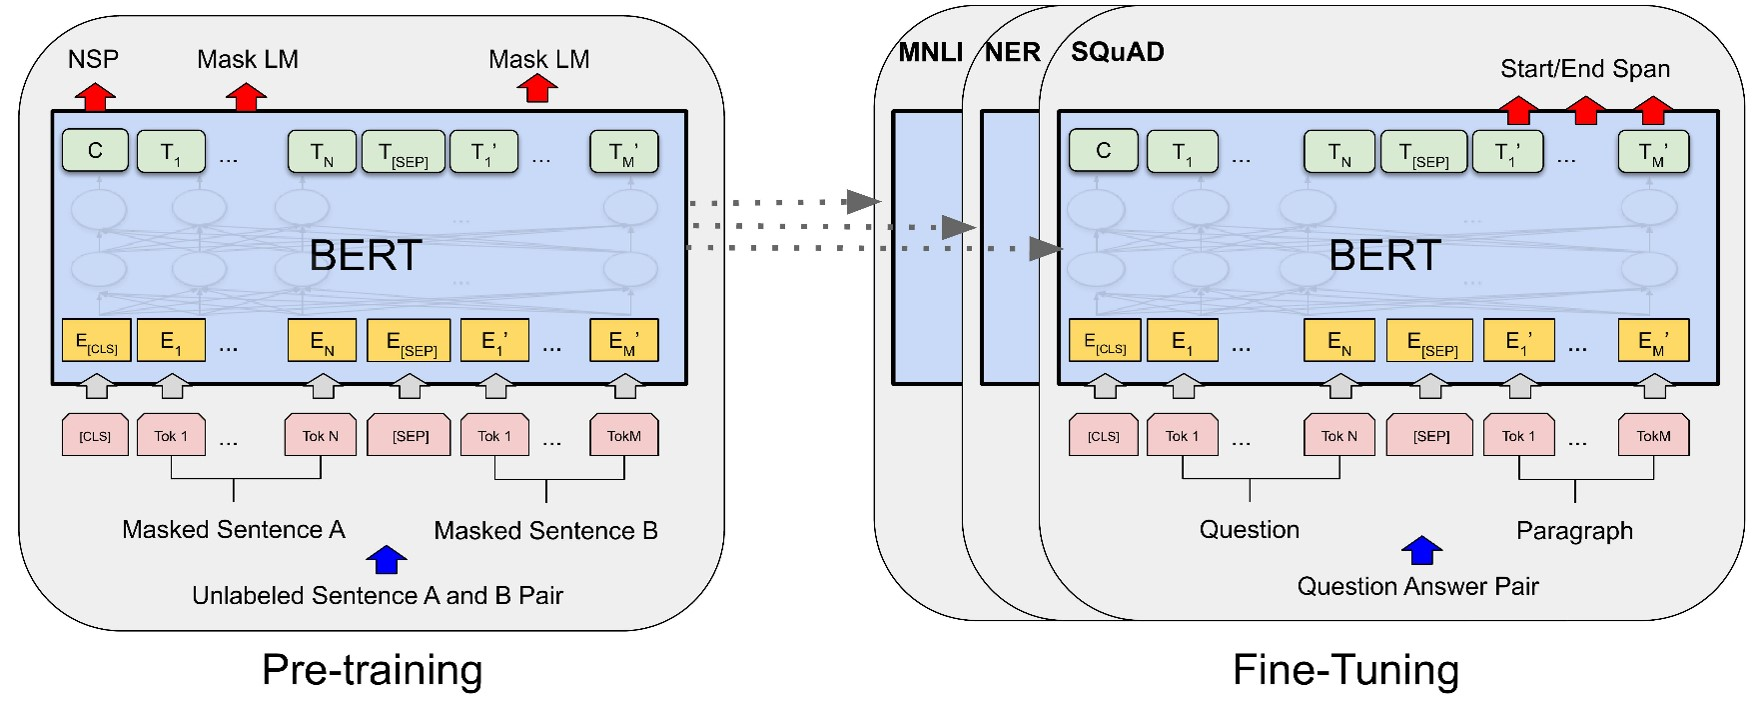
\includegraphics[scale=.9]{img/BERT.jpg} 
% \caption{Toàn bộ tiến trình pretraining và finetuning của BERT.}
% \end{center}
% \end{figure}
% \FloatBarrier
% Chúng ta sử dụng cùng một tham số pretrain để khởi tạo mô hình cho các tác vụ down stream khác nhau. Trong suốt quá trình finetuning thì toàn bộ các tham số của layers học chuyển giao sẽ được fine-tune. Đối với các tác vụ sử dụng input là một cặp sequence (pair-sequence) ví dụ như question and answering thì ta sẽ thêm token khởi tạo là [CLS] ở đầu câu, token [SEP] ở giữa để ngăn cách 2 câu.Tiến trình áp dụng finetuning sẽ như sau:
% \begin{enumerate}
% \item Embedding toàn bộ các token của cặp câu bằng các embedding vector từ pretrain model. Các token embedding bao gồm cả 2 token là [CLS] và [SEP] để đánh dấu vị trí bắt đầu của câu hỏi và vị trí ngăn cách giữa 2 câu. 2 token này sẽ được dự báo ở output để xác định các phần Start/End Spand của câu output.
% \item Các embedding vector sau đó sẽ được truyền vào kiến trúc multi-head attention với nhiều block code (thường là 6, 12 hoặc 24 blocks tùy theo kiến trúc BERT). Ta thu được một vector output ở encoder.
% \item Để dự báo phân phối xác suất cho từng vị trí từ ở decoder, ở mỗi time step chúng ta sẽ truyền vào decoder vector output của encoder và vector embedding input của decoder để tính encoder-decoder attention (cụ thể về encoder-decoder attention là gì các bạn xem lại mục 2.1.1). Sau đó projection qua liner layer và softmax để thu được phân phối xác suất cho output tương ứng ở time step .
% \item Trong kết quả trả ra ở output của transformer ta sẽ cố định kết quả của câu Question sao cho trùng với câu Question ở input. Các vị trí còn lại sẽ là thành phần mở rộng Start/End Span tương ứng với câu trả lời tìm được từ câu input.
% \end{enumerate}
% \subsubsection{Masked Language Modeling (MLM)}
% Masked ML là một tác vụ cho phép chúng ta finetuning lại các biểu diễn từ trên các bộ ngữ liệu unsupervised-text bất kỳ. Chúng ta có thể áp dụng Masked ML cho những ngôn ngữ khác nhau để tạo ra biểu diễn embedding cho chúng.
% \begin{figure}[!htb]
% \begin{center}
% \includegraphics[scale=.35]{img/mlm.png}
% \caption{ Sơ đồ kiến trúc BERT cho tác vụ MLM}
% \end{center}
% \end{figure}
% Theo đó : 
% \begin{itemize}
%     \item Khoảng 15 \% các token của câu input được thay thế bởi [MASK] token trước khi truyền vào model đại diện cho những từ bị che dấu (masked). Mô hình sẽ dựa trên các từ không được che (non-masked) dấu xung quanh [MASK] và đồng thời là bối cảnh của [MASK] để dự báo giá trị gốc của từ được che dấu. Số lượng từ được che dấu được lựa chọn là một số ít (15\%) để tỷ lệ bối cảnh chiếm nhiều hơn (85\%).
% \item Bản chất của kiến trúc BERT vẫn là một mô hình seq2seq gồm 2 phase encoder giúp embedding các từ input và decoder giúp tìm ra phân phối xác suất của các từ ở output. Kiến trúc Transfomer encoder được giữ lại trong tác vụ Masked ML. Sau khi thực hiện self-attention và feed forward ta sẽ thu được các vector embedding ở output là  O\textsubscript{1}, O\textsubscript{2},..., O\textsubscript{5}.
% \item Để tính toán phân phối xác suất cho từ output, chúng ta thêm một Fully connect layer ngay sau Transformer Encoder. Hàm softmax có tác dụng tính toán phân phối xác suất. Số lượng units của fully connected layer phải bằng với kích thước của từ điển.

% \item Cuối cùng ta thu được embedding vector của mỗi một từ tại vị trí MASK sẽ là embedding vector giảm chiều của vector  sau khi đi qua fully connected layer như mô tả trên hình vẽ bên phải.
% \end{itemize}
% \subsubsection{Next Sentence Prediction (NSP)}
% Đây là một bài toán phân loại học có giám sát với 2 nhãn. Input đầu vào của mô hình là một cặp câu (pair-sequence) sao cho 50\% câu thứ 2 được lựa chọn là câu tiếp theo của câu thứ nhất và 50\% được lựa chọn một cách ngẫu nhiên từ bộ văn bản mà không có mối liên hệ gì với câu thứ nhất. Nhãn của mô hình sẽ tương ứng với IsNext khi cặp câu là liên tiếp hoặc NotNext nếu cặp câu không liên tiếp.
% Cũng tương tự như mô hình Question and Answering, chúng ta cần đánh dấu các vị trí đầu câu thứ nhất bằng token [CLS] và vị trí cuối các câu bằng token [SEP]. Các token này có tác dụng nhận biết các vị trí bắt đầu và kết thúc của từng câu thứ nhất và thứ hai.
% \begin{figure}[!htb]
% \begin{center}
% \includegraphics[scale=.7]{img/NSP.png}
% \caption{Sơ đồ kiến trúc model BERT cho tác vụ NSP.}
% \end{center}
% \end{figure}
% \newline
% Thông tin input được preprocessing trước khi đưa vào mô hình huấn luyện bao gồm:
% \begin{itemize}
%     \item Ngữ nghĩa của từ (token embeddings): Thông qua các embedding vector cho từng từ. Các vector được khởi tạo từ pretrain model.
% \end{itemize}
% Ngoài embedding biểu diễn từ của các từ trong câu, mô hình còn embedding thêm một số thông tin:
% \begin{itemize}
%     \item Loại câu (segment embeddings): Gồm hai vector là  nếu từ thuộc câu thứ nhất và  nếu từ thuộc câu thứ hai.
% \item Vị trí của từ trong câu (position embedding): là các vector . Tương tự như positional embedding trong transformer.
% \end{itemize}
% Véctơ input sẽ bằng tổng của cả ba thành phần embedding theo từ, câu và vị trí.

\subsection{Kiến trúc mô hình ViHealthBERT}
\subsubsection{Transformer và BERT}
Mô hình Transformer ứng dụng cơ chế self-attention và multi-head attention được giới thiệu lần đầu trong paper Attention is All You Need\cite{DBLP:journals/corr/VaswaniSPUJGKP17}. 
\begin{figure}
\centering
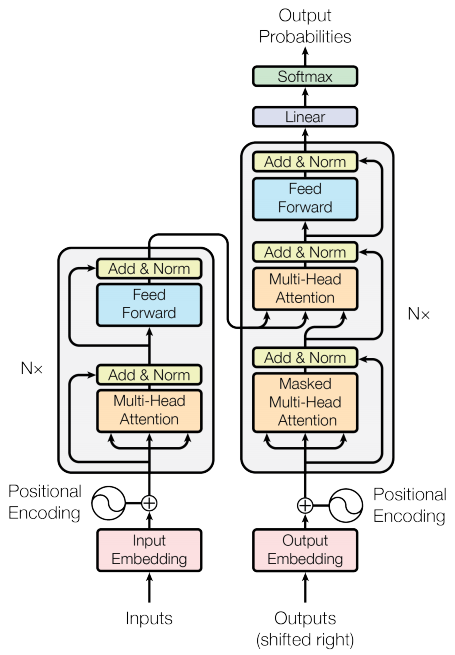
\includegraphics[scale=.35]{img/transformer.png}
\caption{Kiến trúc Transformer\cite{DBLP:journals/corr/VaswaniSPUJGKP17}}
\label{fig:transformer_diagram}
\end{figure}
Phần Encoder của Transformer được sử dụng trong mô hình BERT (\textbf{B}idirectional \textbf{E}ncoder \textbf{R}epresentations from \textbf{T}ransformers)\cite{devlin-etal-2019-bert}. Trong bài báo, BERT được giới thiệu có 2 phiên bản với các siêu tham số (hyperparameters) và số lượng tham số huấn luyện (training parameters) khác nhau:
\begin{itemize}
\item \textbf{BERT\textsubscript{base}}: 12 Transformer encoder layers, 768 hidden units, 12 attention heads, 110 triệu parameters.
\item \textbf{BERT\textsubscript{large}}: 24 Transformer encoder layers, 1024 hidden units, 16 attention heads và 340 triệu parameters.
\end{itemize}
\begin{figure}
\centering
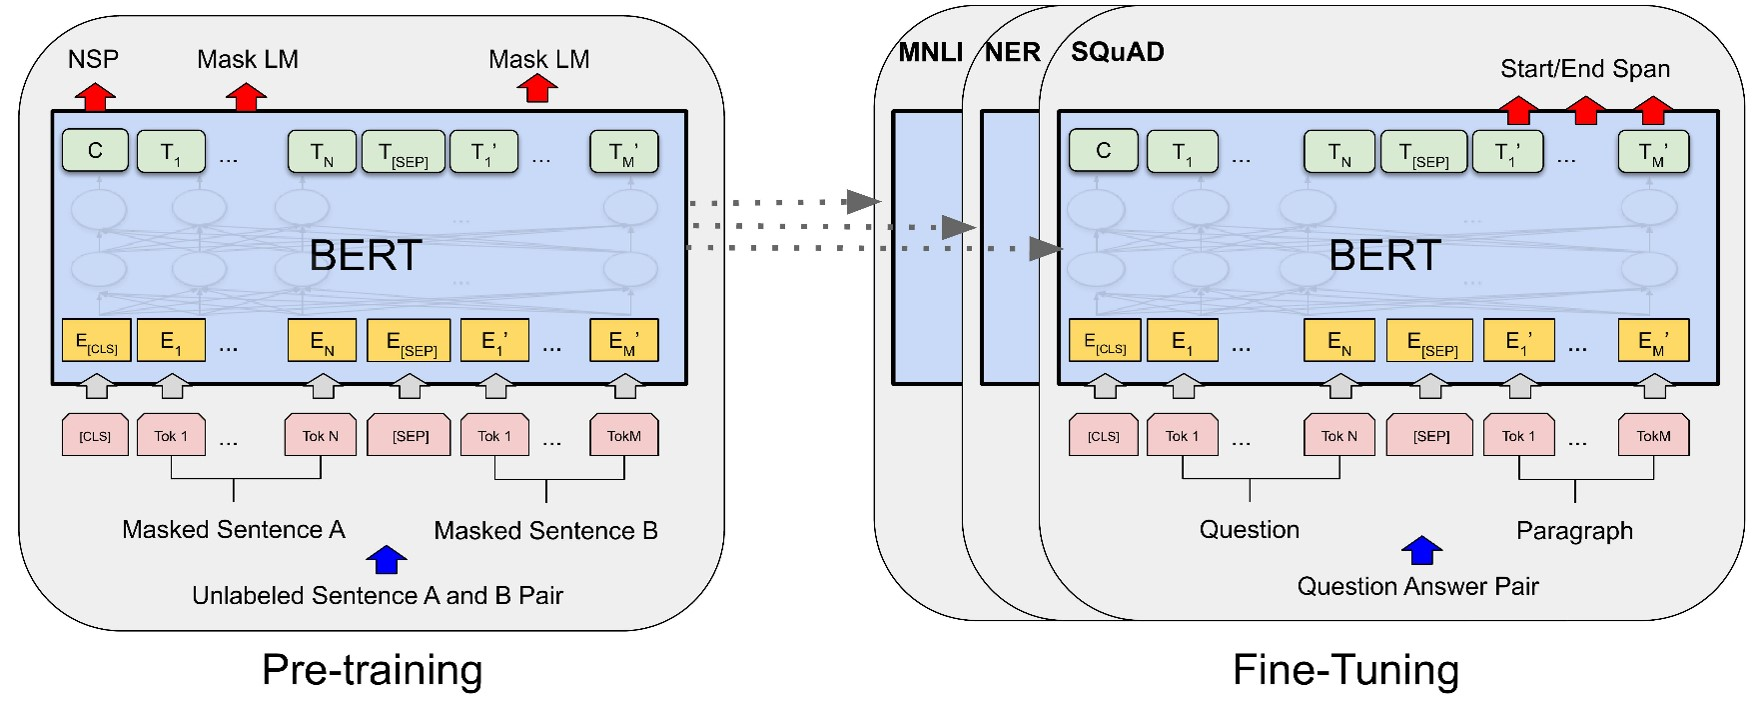
\includegraphics[scale=.65]{img/BERT.jpg}
\caption{Mô hình BERT\cite{devlin-etal-2019-bert}}
\label{fig:my_label}
\end{figure}
BERT được tiền huấn luyện (pretraining) với bộ ngữ liệu \textit{BookCorpus} (800 triệu từ) và \textit{Wikipedia English} (2500 triệu từ), sau đó tinh chỉnh (finetune) lại cho từng task khác nhau. Sau khi BERT được công bố, nhiều mô hình cải tiến của BERT cũng được giới thiệu dựa trên kiến trúc của BERT, trong đó có thể kể đến
\begin{itemize}
\item \textbf{RoBERTa} (\textbf{R}obustly \textbf{o}ptimized \textbf{BERT} Pretraining \textbf{a}pproach)\cite{DBLP:journals/corr/abs-1907-11692}: sử dụng dynamic masking so với sử dụng static masking trong kiến trúc gốc; huấn luyện trên nhiều ngữ liệu hơn.
\item \textbf{DistilBERT}\cite{DBLP:journals/corr/abs-1910-01108}: mô hình nhỏ, nhanh, tốn ít chi phí huấn luyện hơn mô hình BERT gốc: có ít hơn 40\% parameters, chạy nhanh hơn 60\% nhưng hiệu quả bằng 95\% so với mô hình gốc.
\end{itemize}

\subsubsection{PhoBERT}
Dựa trên mô hình BERT, nhóm nghiên cứu từ VinAI đã công bố PhoBERT\cite{phobert}, được giới thiệu là mô hình ngôn ngữ đơn ngữ dành cho tiếng Việt có quy mô lớn đầu tiên. PhoBERT sử dụng quá trình pretraining của RoBERTA để tăng hiệu quả cho mô hình. Kiến trúc của PhoBERT vẫn giữ nguyên so với BERT:
\begin{itemize}
\item \textbf{PhoBERT\textsubscript{base}}: 12 encoder layers, 768 hidden units, 12 attention heads, 135 triệu parameters.
\item \textbf{PhoBERT\textsubscript{large}}: 24 encoder layers, 1024 hidden units, 16 attention heads và 370 triệu parameters.
\end{itemize}
PhoBERT được pretrain với bộ ngữ liệu \textit{Wikipedia Tiếng Việt} và bộ ngữ liệu tin tức tiếng Việt \textit{Binhvq News Corpus}

\subsubsection{ViHealthBERT}
Mô hình ViHealthBERT sử dụng kiến trúc của BERT (12 encoder layer, 768 hidden units, 12 attention heads) với bộ trọng số huấn luyện của PhoBERT. Việc huấn luyện ViHealthBERT chia làm 2 giai đoạn:
\begin{itemize}
\item \textbf{Giai đoạn pretraining}: Huấn luyện trên các bộ ngữ liệu \textit{Text Mining Corpus} và \textit{OSCAR} : Masked Language Modeling (MLM), Capitalized Prediction (CP) và Next Sentence Prediction (NSP).
\item \textbf{Giai đoạn finetuning}: Finetuning trên các bộ ngữ liệu \textit{PhoNER\_COVID-19, VimQ, arcDrid} và \textit{FAQ Summarization}: Named-Entity Recognition (NER), Acronym Disambiguation và FAQ Summarization
\end{itemize}
\begin{figure}
\begin{center}
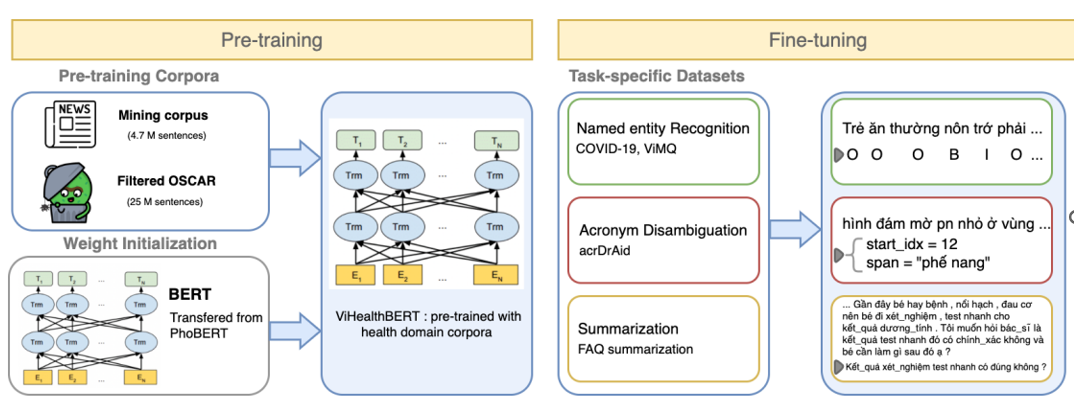
\includegraphics[scale=.8]{img/ViHealthBERT.png}
\caption{Tổng quan về quá trình pretraining và finetuning trong ViHealthBERT\cite{minh-EtAl:2022:LREC}}
\end{center}
\end{figure}

\section{Ứng dụng mô hình ViHealthBERT xây dựng công cụ trích xuất danh sách triệu chứng từ miêu tả của bệnh nhân}
\subsection{Động lực}
Một số bệnh viện có thiết lập hệ thống tư vấn bệnh trực tuyến: người bệnh gửi thông tin cá nhân cùng miêu tả triệu chứng, bác sĩ sẽ đọc và đưa ra chẩn đoán dựa trên miêu tả của người bệnh. Tuy nhiên, đôi khi người bệnh đưa ra nhiều thông tin không liên quan, trong khi bác sĩ chỉ cần danh sách các triệu chứng cụ thể để biết được bệnh nhân đang gặp vấn đề gì.

Nhóm đề xuất sử dụng mô hình ViHealthBERT ứng dụng vào bài toán Medical Named Entity Recognition (Medical NER) Tiếng Việt để tự động trích xuất danh sách các triệu chứng từ miêu tả của bệnh nhân, giúp tăng hiệu suất làm việc ở các cơ sở khám chữa bệnh.

\subsection{Finetune mô hình ViHealthBERT cho tác vụ NER}
\subsubsection{Ngữ liệu huấn luyện}
Nhóm tiến hành finetune lại mô hình ViHealthBERT để giải quyết bài toán Medical NER Tiếng Việt trên tập ngữ liệu PhoNER\_COVID19\cite{truong-etal-2021-covid}. Bộ ngữ liệu có các thông số được trình bày trong bảng~\ref{tab:covid-ner-vietnamese-stats}
\begin{table}
\centering
\begin{tabular}{|l|l|l|l|l|l|}
\hline
\textbf{Entity type} & \textbf{Train} & \textbf{Valid} & \textbf{Test} & \textbf{All} \\
\hline
PATIENT\_ID & 3240 & 1276 & 2005 & 6521 \\
\hdashline
PERSON\_NAME & 349 & 188 & 318 & 855 \\
\hdashline
AGE & 682 & 361 & 582 & 1625 \\
\hdashline
GENDER & 542 & 277 & 462 & 1281 \\
\hdashline
OCCUPATION & 205 & 132 & 173 & 510 \\
\hdashline
LOCATION & 5398 & 2737 & 4441 & 12576 \\
\hdashline
ORGANIZATION & 1137 & 551 & 771 & 2459 \\
\hdashline
SYMPTOM \& DISEASE & 1439 & 766 & 1136 & 3341 \\
\hdashline
TRANSPORTATION & 226 & 87 & 193 & 506 \\
\hdashline
DATE & 2549 & 1103 & 1654 & 5306 \\
\hline
\# Entities in total & 15767 & 7478 & 11735 & 34984 \\
\hline
\# Sentences in total & 5027 & 2000 & 3000 & 10027 \\
\hline
\end{tabular}
\caption{Các thông số của tập ngữ liệu PhoNER\_COVID19\cite{truong-etal-2021-covid}}
\label{tab:covid-ner-vietnamese-stats}
\end{table}

\subsubsection{Thông số huấn luyện và kết quả}
Các thông số huấn luyện được mô tả trong bảng~\ref{tab:configurations}. Nhóm sử dụng các độ đo Precision, Recall và F1-Score để đánh giá kết quả huấn luyện. Với \textit{TP} là số lượng mẫu đúng được dự đoán đúng (True Positive), \textit{FP} là số lượng mẫu đúng nhưng được dự đoán sai (False Positive) và \textit{FN} là số lượng mẫu sai và được dự đoán sai (False Negative). Công thức tính Precision, Recall và F1-Score được định nghĩa như sau:
\begin{equation*}
\begin{aligned}
Precision (P) &= \frac{TP}{TP + FP} \\
Recall (R) &= \frac{TP}{TP + FN} \\
F1 &= \frac{2PR}{P + R}
\end{aligned}
\end{equation*}

Mô hình sau khi huấn luyện đạt được 95\% Precision, 94\% Recall và 95\% F1-Score khi đối chiếu với tập test của bộ ngữ liệu PhoNER\_COVID-19 đã nhắc ở phần trên. Kết quả huấn luyện của mô hình được mô tả trong bảng~\ref{tab:results-test}.
\begin{table}
\centering
\begin{tabular}{|l|c|}
\hline
\# epochs & 10 \\
\hline
batch size & 16 \\
\hline
seqlen & 70 \\
\hline
learning rate & 5e-5 \\
\hline
dropout rate & 0.1 \\
\hline
\end{tabular}
\caption{Thông số finetune mô hình ViHealthBERT cho tác vụ NER}
\label{tab:configurations}
\end{table}

\begin{table}
\centering
\begin{tabular}{|l|l|l|l|}
\hline
\textbf{label}        & \textbf{precision} & \textbf{recall} & \textbf{f1-score} \\ \hline
DATE                  & 0.9909             & 0.9921          & 0.9915            \\ \hdashline
SYMPTOM\_AND\_DISEASE & 0.9322             & 0.9040          & 0.9179            \\ \hdashline
NAME                  & 0.9073             & 0.9073          & 0.9073            \\ \hdashline
LOCATION              & 0.9529             & 0.9381          & 0.9454            \\ \hdashline
PATIENT\_ID           & 0.9857             & 0.9841          & 0.9849            \\ \hdashline
TRANSPORTATION        & 0.9442             & 0.9637          & 0.9538            \\ \hdashline
GENDER                & 1.0000             & 0.9776          & 0.9887            \\ \hdashline
ORGANIZATION          & 0.9064             & 0.9182          & 0.9123            \\ \hdashline
JOB                   & 0.8659             & 0.8208          & 0.8427            \\ \hdashline
AGE                   & 0.9803             & 0.9681          & 0.9741            \\ \hline
\textbf{micro avg}    & 0.9592             & 0.9497          & 0.9545            \\ \hline
\textbf{macro avg}    & 0.9592             & 0.9497          & 0.9544            \\ \hline
\end{tabular}
\caption{Kết quả finetune mô hình ViHealthBERT cho tác vụ NER trên tập test của bộ ngữ liệu PhoNER\_COVID-19}
\label{tab:results-test}
\end{table}

\subsection{Xây dựng ứng dụng}
Ứng dụng cần nhận biết và trích xuất các triệu chứng bệnh từ đầu vào là văn bản của người dùng. Do vậy, nhóm sẽ trích xuất các từ được gán nhãn \textit{SYMPTOM\_AND\_DISEASE} trong văn bản. Một ví dụ cho input (câu văn miêu tả triệu chứng) và output (danh sách các nhãn của câu) có thể thấy trong hình~\ref{fig:example-result}.
\begin{figure}
\centering
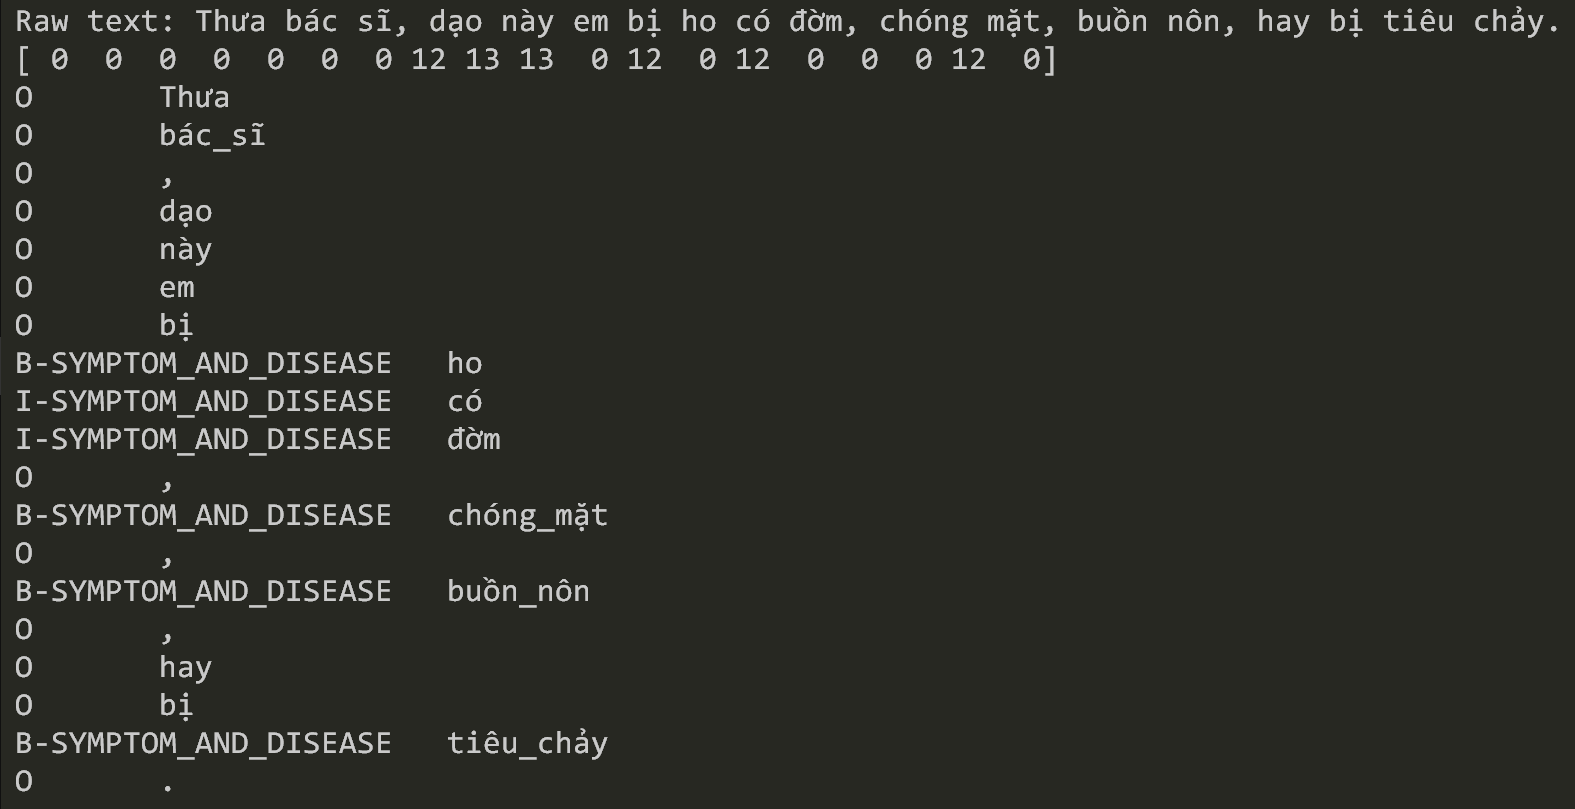
\includegraphics[scale=.5]{img/example-result.png}
\caption{Một ví dụ cho input (câu văn miêu tả triệu chứng) và output (danh sách các nhãn của câu)}
\label{fig:example-result}
\end{figure}

Thuật toán trích xuất các nhãn \textit{SYMPTOM\_AND\_DISEASE} được miêu tả trong Thuật toán \ref{alg:ner-retriever}

\begin{algorithm}
\caption{Thuật toán trích xuất các nhãn \textit{SYMPTOM\_AND\_DISEASE}}
\label{alg:ner-retriever}
\begin{algorithmic}
\Function {RetrieveSymptomsFromNERTags}{\textit{words}, \textit{labels}}
\State $list\_symptoms \gets \{\}$
\State $temp\_symptoms \gets \emptyset$
\State $n \gets |label|$
\For {$i \in [0, n - 1]$}
\If {$labels_i$ = B-SYMPTOM\_AND\_DISEASE}
\If {$temp\_symptoms \neq \emptyset$}
    \State Thêm $temp\_symptoms$ vào $list\_symptoms$
\EndIf
\State $temp\_symptoms \gets words_i$
\ElsIf {$labels_i$ = I-SYMPTOM\_AND\_DISEASE}
\State Thêm $words_i$ vào sau $temp\_symptoms$
\EndIf
\EndFor
\State\Return list\_symptoms
\EndFunction
\end{algorithmic}
\end{algorithm}

Với thuật toán này, nhóm tiến hành xây dựng ứng dụng web cho phép người dùng nhập vào một câu văn (đoạn văn). Dữ liệu được đưa vào mô hình ViHealthBERT đã được finetune để gán nhãn, sau đó bộ nhãn và câu đầu vào sẽ được đưa vào thuật toán đã nêu để trích ra danh sách các triệu chứng. Workflow của ứng dụng có thể được tóm tắt qua hình~\ref{fig:workflow}.
\begin{figure}
\centering
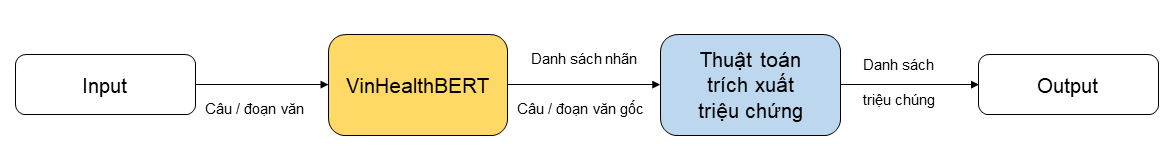
\includegraphics[scale=.6]{img/workflow.png}
\caption{Workflow ứng dụng trích xuất triệu chứng}
\label{fig:workflow}
\end{figure}
Nhóm sử dụng Flask framework để xây dựng ứng dụng web.
%% TODO: more description here
Nhóm xây dựng ứng dụng web bằng Flask framework (backend API) và Flutter (frontend).

\section{Hướng dẫn sử dụng ứng dụng}
\subsection{Cài đặt}

\subsection{Chạy thử}

\section{Tổng kết}
Qua đồ án này, nhóm xin tổng kết lại các nội dung đã thực hiện:
\begin{itemize}
\item Nhóm finetune mô hình ViHealthBERT cho tác vụ NER dùng bộ ngữ liệu PhoNER\_COVID19. Mô hình sau khi finetune đạt được 95\% Precision, 94\% Recall và 95\% F1-Score khi đối chiếu với tập test của bộ ngữ liệu PhoNER\_COVID-19.
\item Từ mô hình đã huấn luyện, nhóm xây dựng một ứng dụng hỗ trợ trích xuất các triệu chứng bệnh từ mô tả của người dùng.
\end{itemize}
Trong tương lai, nhóm đề xuất một số hướng cải tiến ứng dụng nhằm mang lại hiệu quả và trải nghiệm tốt nhất cho người sử dụng. Một số hướng cải tiến nhóm đề xuất bao gồm:
\begin{itemize}
\item Xây dựng một module chẩn đoán bệnh dựa trên danh sách các triệu chứng. Danh sách triệu chứng hiện có sẽ được đưa qua một mạng neural đơn giản (hoặc một mô hình học máy như Conditional Random Fields) để đưa ra chẩn đoán nhanh. Tuy nhiên người bệnh vẫn cần tham khảo ý kiến của bác sĩ để có được chẩn đoán chính xác nhất.
\item Hỗ trợ nhập liệu từ file. Khi đó hệ thống có thể trích xuất và đưa ra danh sách triệu chứng của nhiều bệnh nhân cùng lúc.
\end{itemize}


% \cleardoublepage
\phantomsection
\addcontentsline{toc}{section}{Tài liệu}
\bibliographystyle{apalike}
\bibliography{sample}

\end{document}